\section{叠加与速度分析}
\label{sec:3.5}

按炮检距沿双曲线迸行叠加,可能是地震勘探中最重要的计算机处理过程了。比它偏移
更为重要,因为它使数据库从$(s, g, t)$空间的一个体积简化为$(y, t)$空间的一个平面。
地震资料解释人员现在还很少有人采用计算机化的电影式地震资料,所以大多数解释人员在
他们能解释分析之前都必须使地震资料经过叠加处理。偏移只不过就是把资料从一个平面转
换至另一个平面。此外,偏移有个缺点:有时它把近地表速度横向变化和多次反射造成的混
乱也混杂在一起了。叠加处理也可能混杂有这类影响,不过,在条件恶劣的地区,资料要不
经过叠加处理,那就别想看盅什么东西。除前面列举的各点之外,叠加处理还有个附带的产
品,那就是据此可以估计岩石速度。

从历史上说,曾经采甩射线法来完成叠加处理,而且现在仍然几乎是唯一地按这种方式来
处理。而另一方面,偏移则总是采用波动方程方法来完成,那就是说,以Fourier变换或有
限差分方法来实现。偏移与叠加二者均属涊曲线识别处理过程,偏移时采用波动方程方法有
许多好处,这些好处难道不能同等地适用于益加吗?看起来似乎是应该如此,但是现在的勘
探实践还没有怔实这点,其原因还不太清楚。本章以后各节内容实际上是属于专题研究性
质,其标题不紡戏称为《不久将要建立的理论》。有关速度估计的更高级概念在\ref{sec:5.0}节至\ref{sec:5.4}
节讨论。波动方程叠加与速度测定方法均是独创性方法,它们也许还缉有经受过令人满意的
检验,或者它们也许还只是不完善地被汇总在一起的。给读者留有想像的余地,时间将会告
诉我们究竟如何。

为什么许多这种理论并没在常规勘探工作中应用?可能的一种原因是:为消除冗余信息
而进行叠加这种论点大概更适合于作为一个统计问题来处理,而不能作为一种物理问题来处
理。为考虑到这类随机偶然性,我得多用一点笔墨来讨论“波动方程时差校正”,这是一种
将统计分析推迟到向下延拓处理之后再迸行的方法。另一种可能原因则是:比起波动方程
来,用射线法解决:排列末端数据丢失和雄列长度范围内出现空间假频的问题,大概要更为灵
活。对于这类随机偶然性质,我特意列了简短一小节来讨论数据恢复问题。不论是哪种情
况,本章论述的数据处理办法想来都应有所裨益。

\subsection{正常时差校正(NMO)}
\label{sec:3.5.1}

正常时差校正(NMO)就是对时间轴进行某种拉伸,使所有地震记录看来像是零炮检
距地震记录。\ref{sec:3.0.1}节内曾首先讨论过NMO,在那种最简单的形式中,NMO是以毕达哥拉斯
关系$t_{nmo}^2=t^2-x^2/v^2$为基础的。在地层的速度为恒定时,正常时差校正要取双曲线族的渐
近线并沿它移动直至与$t=0$重合,这就是在时间轴上舍去初至之前的任何采样值,然后再将
地震记录的其余部分拉平。接近初至之处,拉伸影响最为显著,在以后的各时间上则逐次减
弱。在图\ref{fig:vdmo/cmpnmo}所示的正常时差校正例子中,你会注意到有由拉伸而形成的许多低频成分。
\begin{figure}[H]
\centering
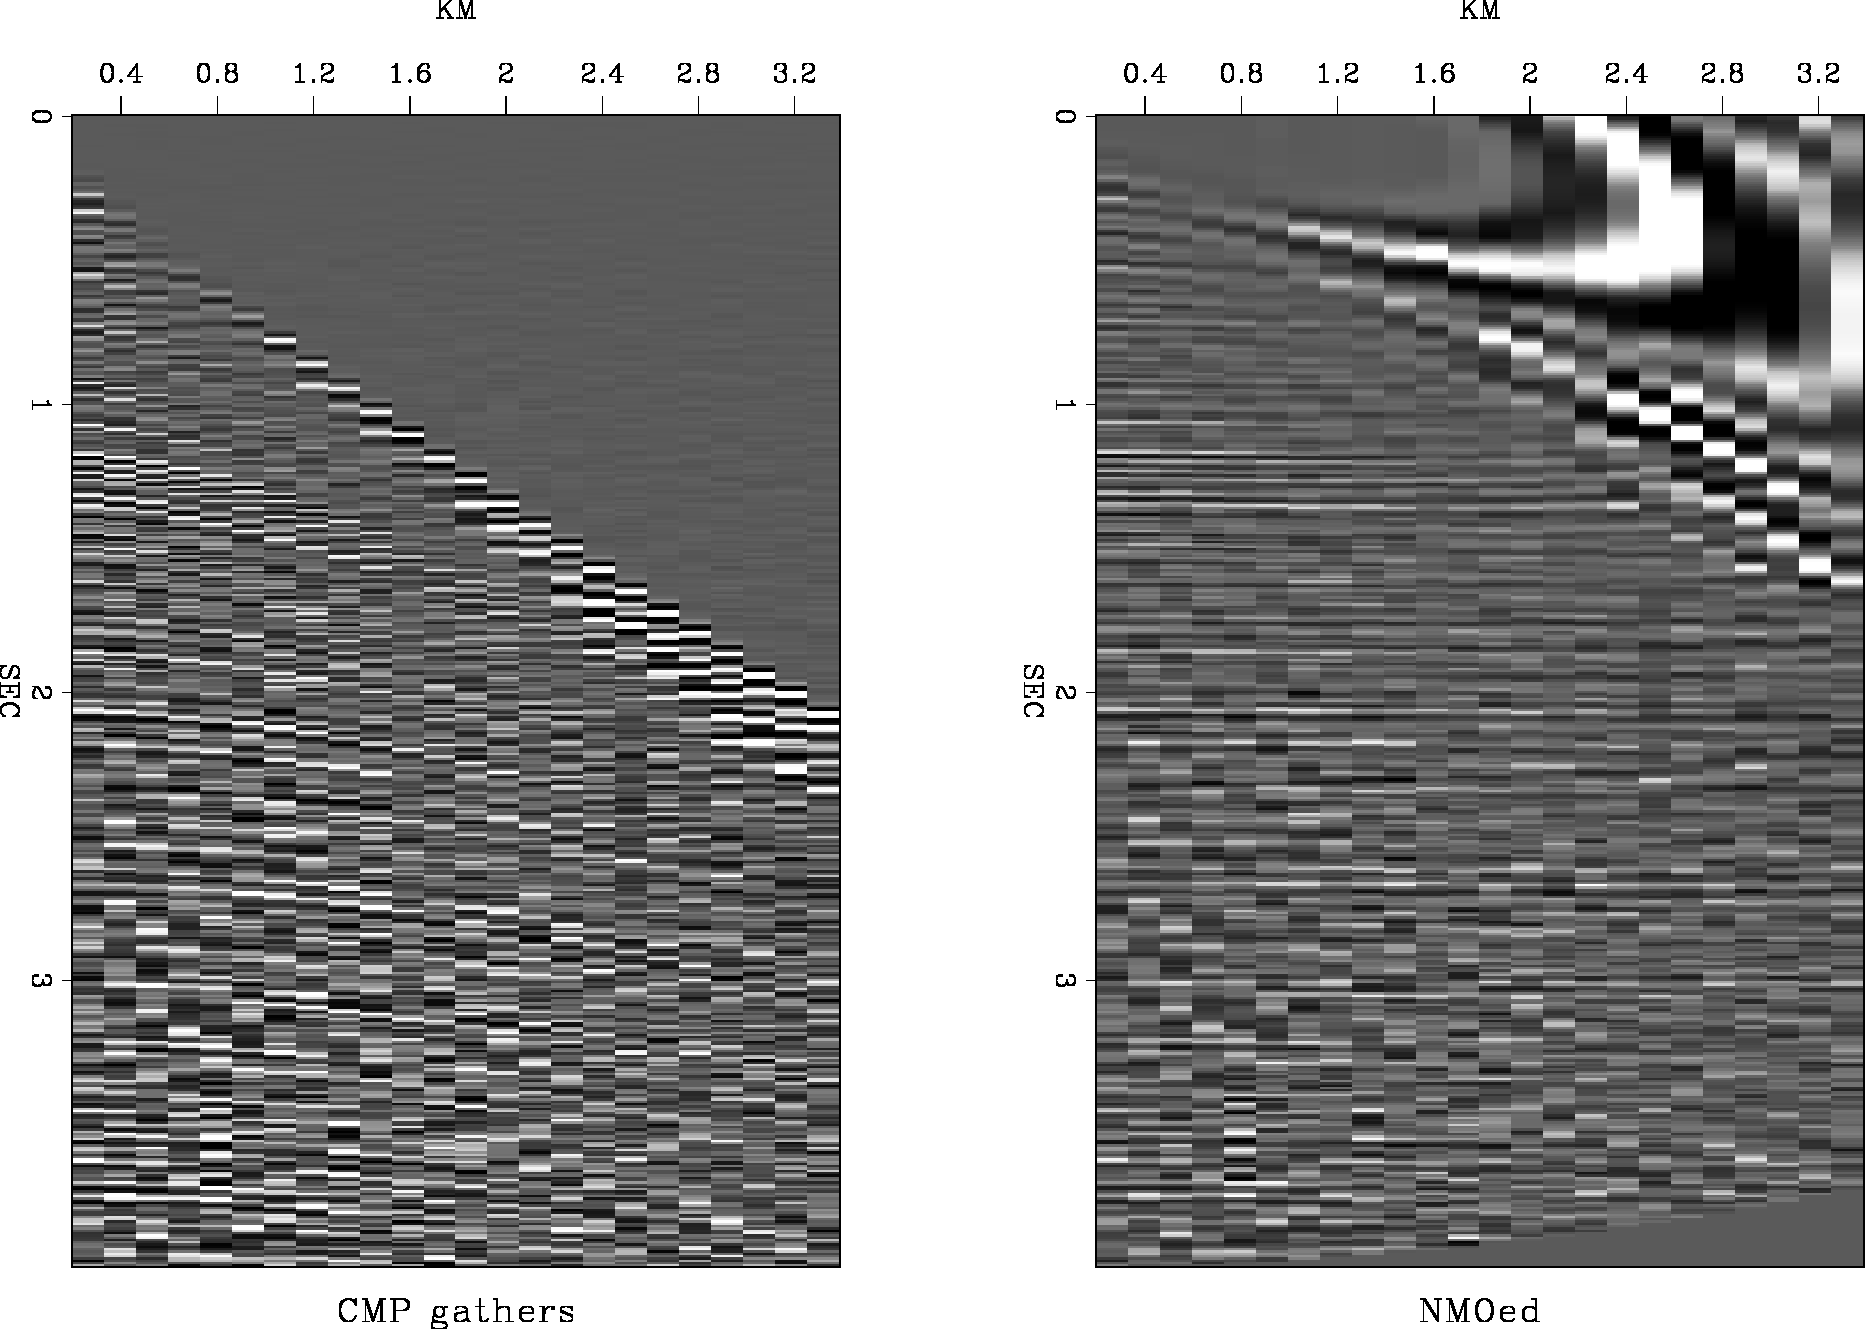
\includegraphics[width=0.65\textwidth]{vdmo/cmpnmo}
\caption[cmpnmo]{左图所示为墨西哥海湾地区的共中心点道集,经正常时差校正后如右图所示}
\label{fig:vdmo/cmpnmo}
\end{figure}

能够作正常时差校正的是共炮点道集或共中心点道集。应用于共炮点道集的正常时差校
正使该道集成为类似于零炮检距时间剖面的一小部分,这时地质构造突出地被展现出来。对共
中心点道集进行正常时差校正,是确定地层的速度与深度之函数关系的主要手段,这是因为共
中心点道集对地层之倾角是不灵敏的。

从数学上说,有关正常时差NMO的变换是一种线性运算。事情看来似乎有些矛盾,一种
非均匀的时间坐标拉伸运算竟是某种线性运算,可是坐标拉伸确实是满足与线性性质有关的
数学条件。不要把流行的线性条件混淆为不太常见的时间不变量条件。线性性质仅要求;对
于将原始数据P分成几部分(例如分成与$P_1$与$P_2$)的任何分解来说,经过正常时差校正的几
部分之和应等于和之正常时差校正。分解的例子包括:(1)分成较早各时间和较晚各时间;
(2)分成偶数时间点和奇数时间点;(3)分成高频和低频;(4)分成大信号值与小信号值。

为把正常时差校正想像成是一种线性算子,试将地震记录考虑为某种向量。NMO算子
类似于一个对角线矩阵,但是沿矩阵对角线分布的是内插滤波因子,而且各内插滤波因子均
有偏离对角线的相移以形成所期望的时延。

\subsection{常规速度分析}
\label{sec:3.5.2}

常规速度分析要利用一系列试验速度,每种试验速度取为深度的恒定函数并用它对数据
进朽时差校正。图\ref{fig:vdmo/cmphale}的左图为用一恒定速度对图\ref{fig:vdmo/cmpnmo}所示共中心点道集进行时差校正之后的结果。注意,该道集中部的各同相额均将近拉平,而较小时间上的同相轴则校正不足,
较大时间上的同相轴则过校正。这种现象很典型,因为正常时差校正量的变化是与速度
呈反比关系(根据毕达哥拉斯关系即可知),而地层的速度在通常情形下正是随深度而增大
的。利用遍及CDP道集各炮检距进行求和的结果作为时差校正速度是否良好拟合于地层速度
的一神测度,大概说来,速度拟合程度越佳,求和值就将越大,用许多种速度重复进行这种
过程,按求和值的幅度绘制等值线图,将它显示为时间与速度的函数,这就是速度谱,如图
\ref{fig:vdmo/cmphale}的右图所示。

\begin{figure}[H]
\centering
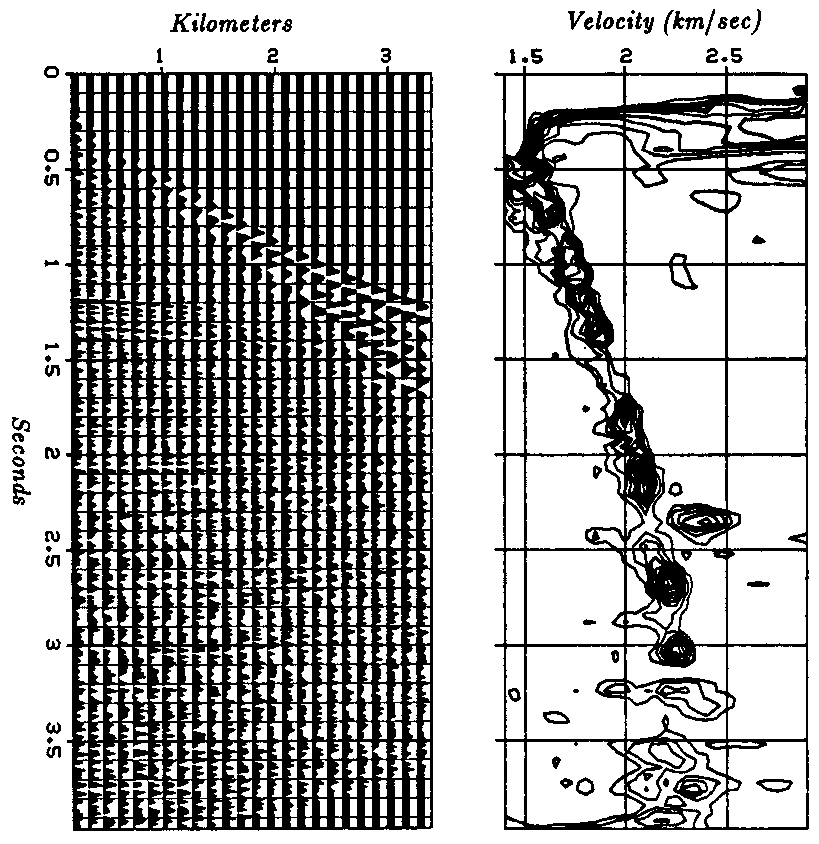
\includegraphics[width=0.65\textwidth]{vdmo/cmphale}
\caption[cmphale]{按恒定速度进行正常时差校正及速度分析结果}
\label{fig:vdmo/cmphale}
\end{figure}

在实际处理时,求和之前可
以采用一些额外的修饰处理步骤。可以按记录道的功率和按它
们的谱(见\ref{sec:5.5}节有关反褶积处理的论述)对各记录道作道间均
衡处理(使它们比例相等)。类似还有,可以将求和所得幅值加
以平滑和归一化(见Taner与 Koehler(l969)的论文)。还可
以如下节所述将数据加以编排和加权。

得出最佳叠加效果的速度是 反射面以上各地层之速度的某一
种平均值,这种平均值的精确定义推迟到\ref{sec:5.4}节再去讨论。

\subsection{切除与加权}
\label{sec:3.5.3}

定义切除函数是常规赴理中
的重要一部分。切除函数就是用 于压制掉数据中某些不希望要的
部分时所使用的一种加权函数。图\ref{fig:vdmo/mute}所示是经过切除处理之野外剖面的例子。加权与切
除对叠加的质量有重大影晌。因此,有许多试验和理论讨论实际上都是以它们作为研究主
题,这是毫不奇怪的。

\begin{figure}[H]
\centering
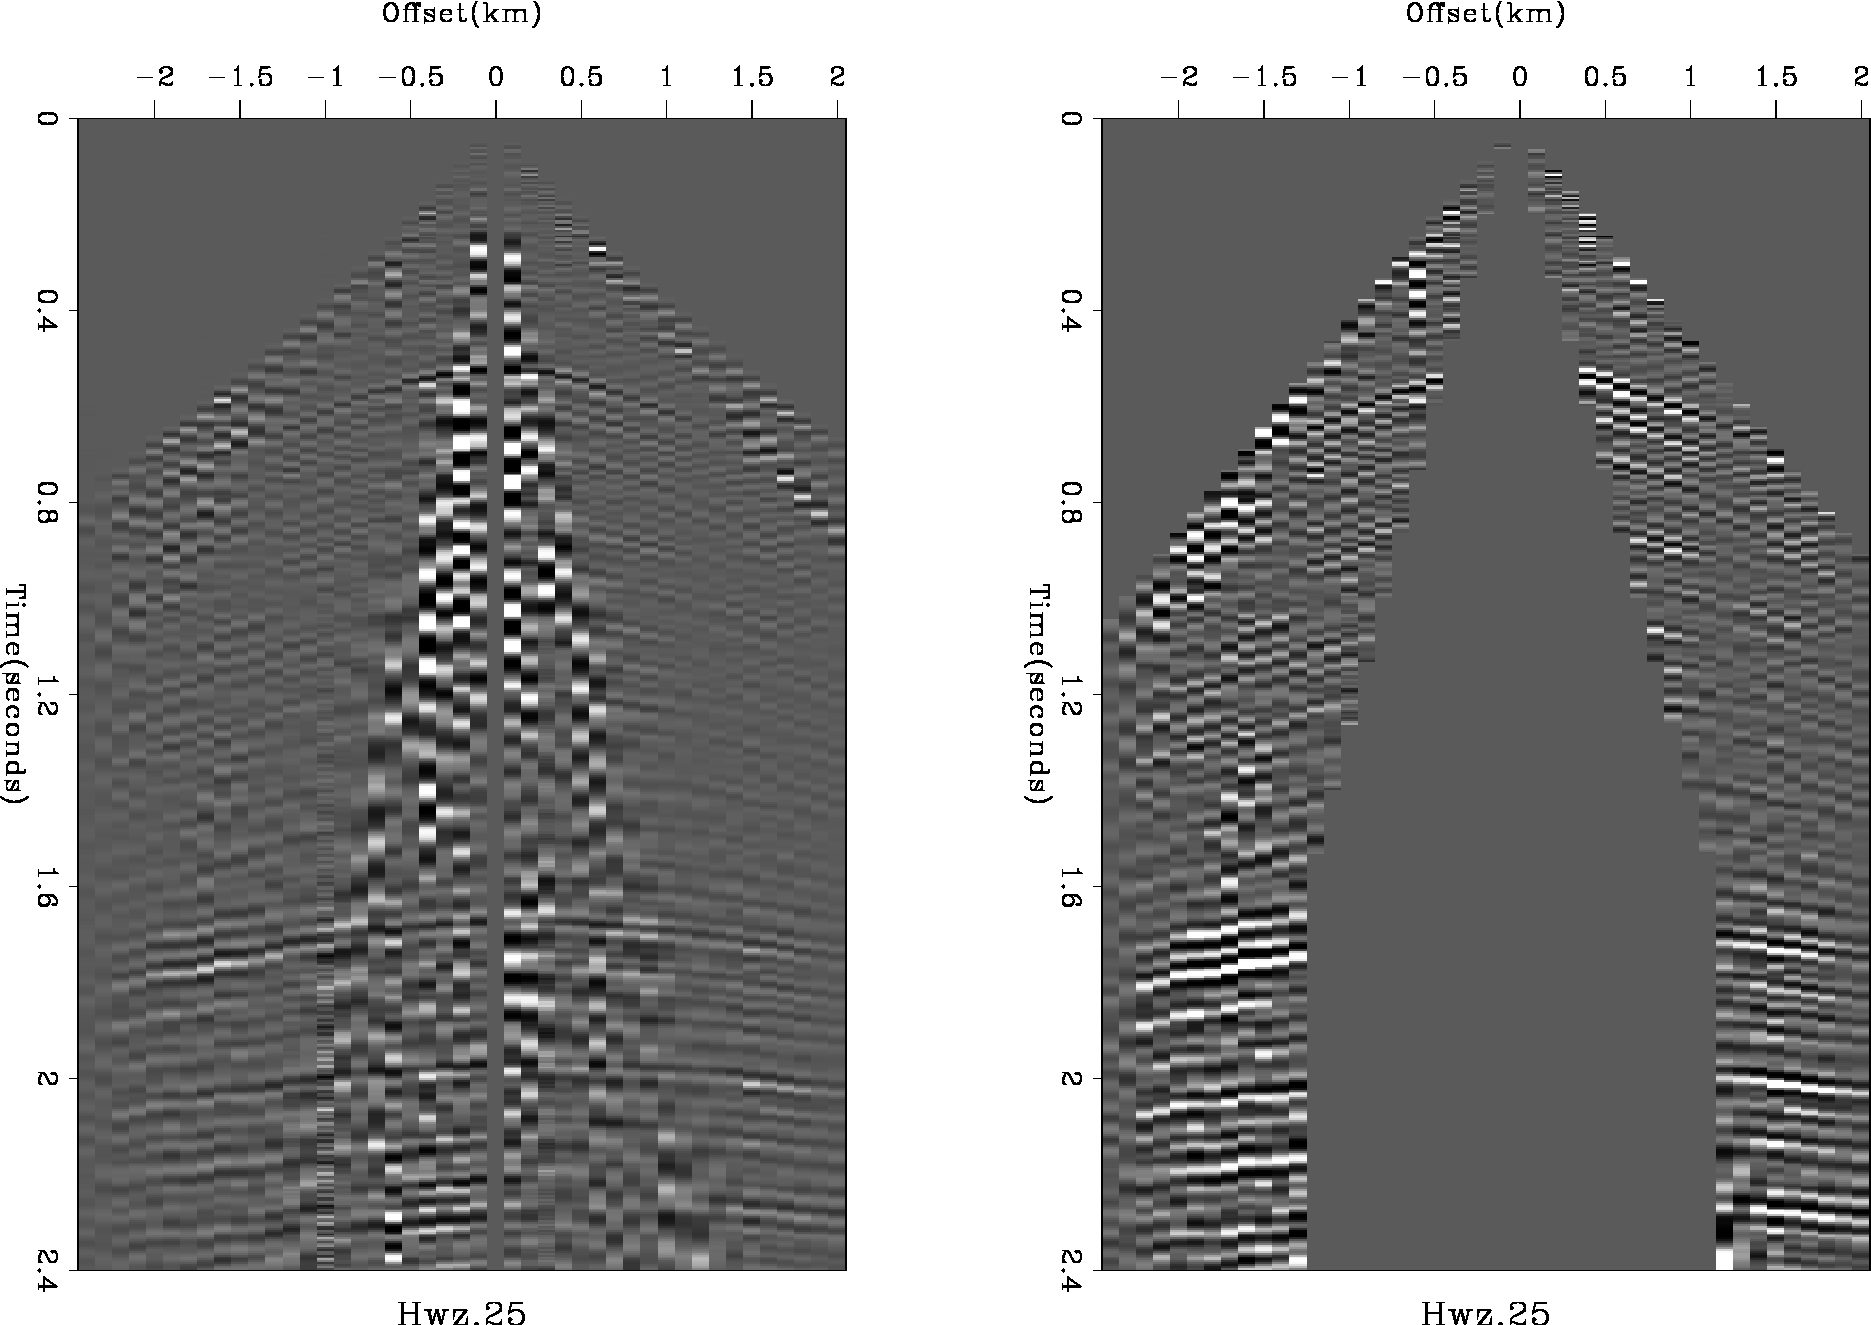
\includegraphics[width=0.65\textwidth]{vdmo/mute}
\caption[mute]{左图是Alberta地区的陆地勉震记录,右图是该记录经过切除处理后
的结果,地滚波(记录中部)与首波(第一个波至)均已消除}
\label{fig:vdmo/mute}
\end{figure}

切除函数往往是以r为变量的一维函数,其中\footnote{h为炮检距,t为时间.------译者},$r=h/t$。 既切除大r值时的数据也切除小r值时的数据,其原因如下所述。

在小r值时,炮点附近仍然可发现有能量存在,诸如水或泥块坠落所形成的影响,或者
低速地滚波所形成的干扰能量。

r值大时,则存在与初至有关的问题。在这种情形下,正常时差拉伸最大而且对速度极
敏感。这初至往往称作首波或折射波。从野外观测看,首波就是一种其旅行时间表现为距离
之线性函数的波。就理论上考虑,针对分层介质很容易对首波作出解释。首波具有沿一地层
边界面作水平传播的射线。在实际现象中,首波可以弱于或者是强于反射波,首波强于反射
波可以用反射波作三维分布而首波仅作二维分布这个事实来解释。

可以把切除楚理看作是用零值迸行加权。为产生最有利的叠加效果,可以选择更普遍性
的加权办法。完善的分析肯定应将干扰噪音和截断影响考虑在内,我们权且作一个简化分析
吧,它可导出最基本的加权函数。

一般我们是沿双曲线遍及所有炮检距进行求积。考虑三维问题时则与此不同,你这时实
际是希望遍及一旋转双曲面进行求积,假设该双曲面是呈径向对称的,按炮检距h的大小对
被积函数进行加权,就使得通常的线性积分能够模拟出遍及旋转双曲面的积分结果
\footnote{这是必须迸行加权处理的第一个理由.所谓沿双曲线的积分,实即正常时差校正并叠加;所罚沿旋转双曲面求
积,就是考虑球面扩散影响时的叠加。因此,必须按炮检距的大小,成比例地对叠加道(所谓被积函数)进行加权,校正
该种影响,这时的叠加处理(所谓的线性积分)结果,才能消除三维情形下的能量扩散。直接了当地说,进行加权处理的
第一个理由就是必须对波阵面球面扩散影响进行适当的补偿。}。叠加
前要按炮检距h的大小对数据进行按比例放大,还有第二个原因,那就是在零炮检距附近能
获得的速度信息不多,这些记录道的时差很小而在远炮检距时则可获得很多速度信息,这些
记录道的比值比较大
\footnote{这是必须进行加权处理的第二个理由。浅显地说,近炮点记录道时差小,因而速度分辨率低;远炮点记录道时差
大,速度分辨率高。但是近炮点记录道振幅强,而远炮点记录道因能量衰减而振幅弱,采用以叠加方法为基础的速度分析
时,将因此而主要是反映近炮点记录道的作周和影响,降低了速度分析的精度。因此必须按炮检距的大小而成比例地加权
放大记录道辐值,使得近炮点与远炮点记录道的振幅在叠加中发挥同等作用。这种加权处理,对远度谱而言,可提高速度
分辨率;对叠加处理来说,可提高叠加效果和质量。-译者}。

% \subsection{Cheops金字塔}
% \label{sec:3.2.4}

% 由于点散射模型之重要性,我们将求助于各种长度关系,以便使式\ref{eq:ex3.2.3}中的$t$、$z$、
% $x$、$s$与$g$之间的函数关系具体可见。利用一维图形来表示这种反映爆炸反射面几何形态的圆
% 锥曲线剖面是非常困难的。

% 首先,假设式\ref{eq:ex3.2.3}中的第一个平方根式是常数,因为现在令其中任何项均保持为
% 常数。这样,就剩下$(g,t)$空间内熟悉的双曲线了,除了对时间已经加上一个常数以外。
% 相反,再假设另一项平方根值为常数,类似地由此又得出$(s,t)$空间内的一个双曲线。在
% $(s,g)$空间内,旅行时间等于$s$的一个函数加上$g$的一个函数。我想,这图像有点像是一个
% 平行于$s$轴的衣架,同另一个平行于J轴的衣架柑交地悬挂着。

% 旅行时间与各坐标的关系图形犹如是耸立在$(s,g)$平面上或者$(y,h)$平面上的一座山。如
% 图\ref{fig:ofs/cheop}(a)所示。注意,在大$t$时通过该山的一个横切面是方形的,方形的各角已经加以平
% 滑。 一个恒定的$t$值就相应于$(s,g)$空间内的一个方形等高线,如图\ref{fig:ofs/cheop}(b)所示。从代
% 数上说,在一个点反射体接近于地表面的情形下,例如当$z\rightarrow 0$时,该种方形的性质就变得更
% 为明显,这时,式\ref{eq:ex3.2.3}变为
% \begin{equation}
% vt=\mid s-x \mid + \mid g-x\mid
% \label{eq:ex3.2.4}
% \end{equation}
% 该正方形之中心位于$(s,g)=(x,x)$。令旅行时间$t$沿垂直于$(s,g)$空间内的水平面的
% 方向向下增大,则相应的方形等高线形状看起来就像是通过埃及Cheops金字塔的一个水平切片
% 一般。在一定高度环绕该金字塔走一圈,就是环绕方形走一圈。从另一种角度看,在
% $s$为恒定的情形下,沿$g$方向横穿过该金字塔时的高度变化,简单就是一个常数加上一个绝对
% 值函数,保持恒定而沿$s$方向横穿过时的情形也是一样。
% \begin{figure}[H]
% \centering
% 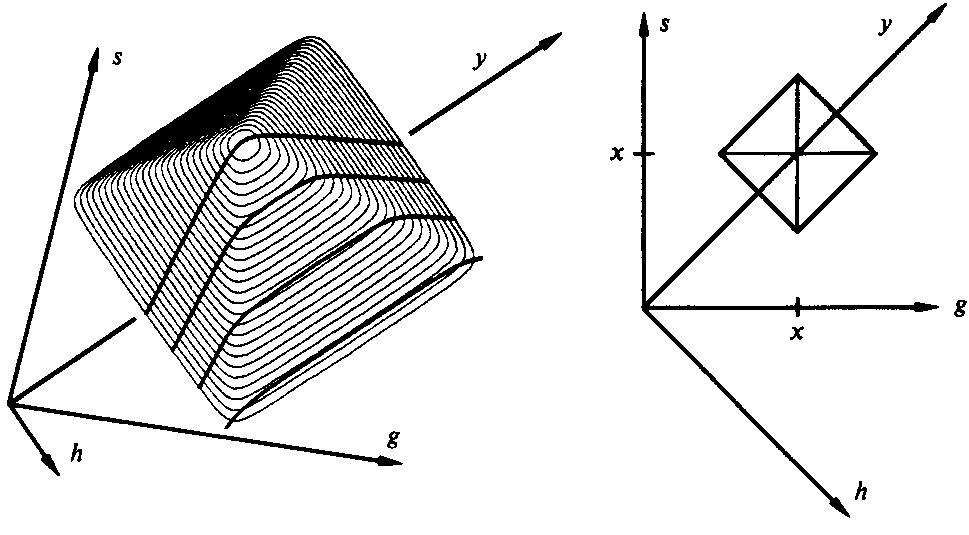
\includegraphics[width=0.65\textwidth]{ofs/cheop}
% \caption[cheop]{(a)图为方程\ref{eq:ex3.2.3}在$x$和$z$固定时的旅行时间图像,
% 看起来像一座山,其中,粗黑线是恒定炮检距剖面。(b)图
% 为大$t$时(或小$z$时)通过该山的一个横断面}
% \label{fig:ofs/cheop}
% \end{figure}
% 更为有趣但不显而易见的情形是共中心点道集的各种曲线和恒定炮检距剖面。回想一
% 下,根据定义,位于炮点与检波点之间的中心点其坐标为力$y$;再有,$h$等于从炮点至检波点
% 的水平偏移距离的二分之一
% \begin{subequations}
% \begin{equation}
% y=\frac{g+s}{2}
% \label{eq:ex3.2.5a}
% \end{equation}
% \begin{equation}
% h=\frac{g-s}{2}
% \label{eq:ex3.2.5b}
% \end{equation}
% \label{eq:ex3.2.5}
% \end{subequations}
% $h$恒定时,沿$y$方向的横截面如图\ref{fig:ofs/cheop}所示。在该横截面的最高处,你是在一个如图\ref{fig:ofs/twopoint}秃
% 顶双曲面的平坦水平阶地上行走。金字塔的顶部和各凌角经受某种侵蚀而被平滑后,就很像
% 是非零反射面深度情形下的这么一种模型。

% 在各射线均接近于垂直的情形下,时距曲线均远离双曲线之渐近线,这时式\ref{eq:ex3.2.3}
% 中的各平方根均可按Taylor级数展开,近似代表一个旋转拋物面,金字塔受侵蚀的顶部形
% 状可用此描述。

% \subsection{随机分布的点散射}
% \label{sec:3.2.5}

% 图\ref{fig:ofs/randcos}所示是取自大约包含有五十个随机分布点散射体所形成之地层模型的一个合成
% 共炮检距时间剖面(COS),其中到达时间较晚者呈双曲线形,早到达者则双曲线具有平坦的
% 顶部。最早到达的可能初至相应于射线水平地从炮点直接到达检波点。
% \begin{figure}[H]
% \centering
% 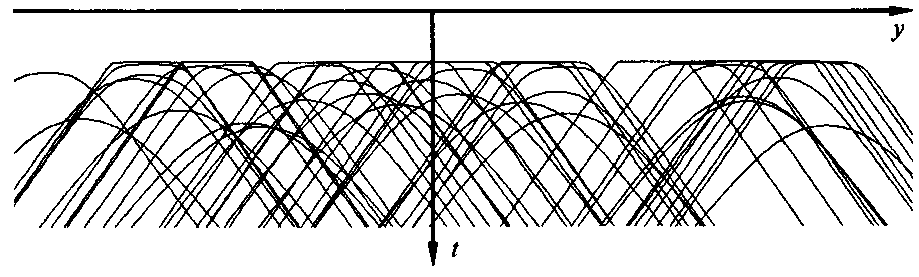
\includegraphics[width=0.65\textwidth]{ofs/randcos}
% \caption[randcos]{随机分布点散射体形成的共炮检距时间剖面}
% \label{fig:ofs/randcos}
% \end{figure}

% 图\ref{fig:ofs/randcsp}所示是由同一个随机分布点散射的地层模型作出的合成共炮点剖面(CSP)。
% 其中,每个散射体均形成一个S曲线型的时距曲线。在零炮检距附近,各双曲线均不对称,
% 它们的位置是随机的,不过,它们必然全都位于各直线$\mid g-s\mid=vt$之下。不但在较早的时间
% 上,而且在较晚的时间上,都可以发现具有尖锐顶部的双曲线。然而,由检波点附近的浅层
% 散射侔所形成的各尖锐顶部必然都位于接近于各直线$\mid g-s\mid=vt$之处。

% \begin{figure}[H]
% \centering
% 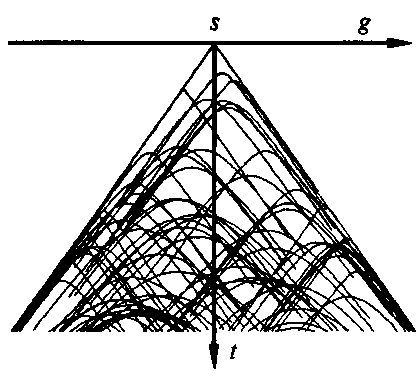
\includegraphics[width=0.65\textwidth]{ofs/randcsp}
% \caption[randcsp]{随机分布点散射体形成的共炮点剖面}
% \label{fig:ofs/randcsp}
% \end{figure}

% 图\ref{fig:ofs/randcmp}的左图所示是由包含有大约五十个随机分
% 布点散射体的一个地层模型所形成的合成共中心点道集
% (CMP)。因为这是一种共中心点道集,各曲线经过零
% 炮检距时均呈对称(野外资料的各负值炮检距从不绘
% 岀)。某些双曲线具有平坦的顶部,这表明相应散射点均非直接位于中心点之下。

% \begin{figure}[H]
% \centering
% 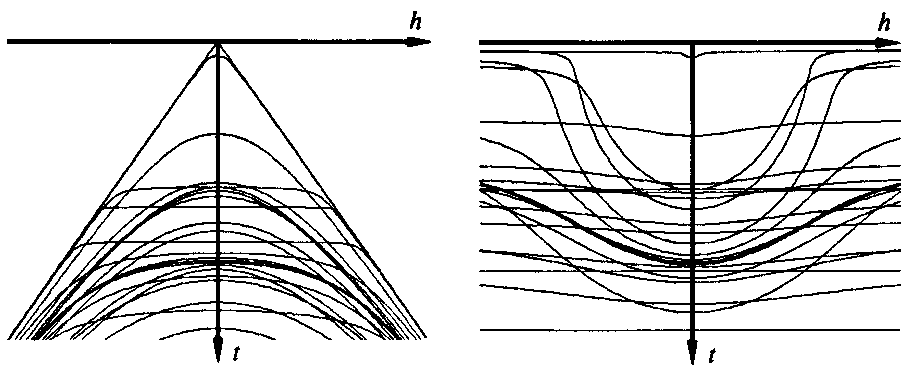
\includegraphics[width=0.65\textwidth]{ofs/randcmp}
% \caption[randcmp]{随机分布点散射体形成的共中心点道集(左图)。同一
% 道集经过时差校正之后的情形(右图)}
% \label{fig:ofs/randcmp}
% \end{figure}

% 正常时差校正是对数据资料进行拉伸处理,试图使
% 馭曲线变成平缓,这种校正要求地层要平坦,但是对于
% 直接位于中心点之下的点散射体,这种处理也是有效
% 的。图\ref{fig:ofs/randcmp}的右图表示对随机散射体模型应用正常
% 时差校正时会发生什么现象,这时某些反射被展平了,另外一些则“过校正”了。

% \subsection{正向与反向散射:Larner条痕}
% \label{sec:3.2.6}

% 在某些地段上,远地表波(near-surface wave)压制了有地质意义的深层反射。由于
% 地表面比起下面较深地层更为大大地不规则,所以近地表波通常均不规则,这使得我们的困
% 难复杂化了。在陆地上,这些干涉波称作地滚波;在海上,它们称作水波(water wave),
% 但别把它们与水面上的表面波相混。

% 图\ref{fig:ofs/vertlay}中垂直的反射壁就可能是产生这类近地表干扰的一种模型,在这种模型中,波
% 仍然是靠近地表传播的。随机分布的垂直壁可以形成类似图\ref{fig:ofs/shelikof}所示野外资料那样的零炮
% 检距时间剖面。另一类不太少见的近地表干扰模型就是随机点散射模型中的平顶曲线了。

% \begin{figure}[H]
% \centering
% 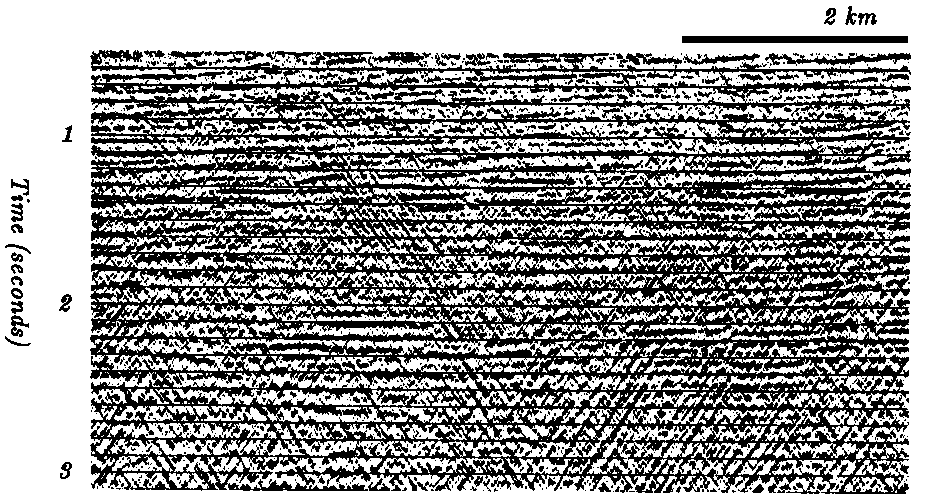
\includegraphics[width=0.65\textwidth]{ofs/shelikof}
% \caption[shelikof]{阿拉斯加地区Slielikof海峡的具有水层干扰之共深度点迭加时间剖面(据Lamer
% ) }
% \label{fig:ofs/shelikof}
% \end{figure}

% 在随机点散射模型中,速度是一项常数。在实际情况下,对近地表波来说,地层速度一
% 般比较低,对深层反射来说,速度一般比较高,这就使放大某种不受欢迎的干扰有了可乘之
% 机。

% 进行共深度点叠加可使具有叠加速度的同相轴得到加强,压制具有其他速度的同相轴。
% 因而你也许会猜想,在较深部位上进行叠加,较高的速度将会压制具有低速度的近地表同相
% 轴。其实大谬不然,近地表干扰都不是从水平地层发生反射;它们倒是非常像是从垂直壁或陡
% 倾斜地层发生的反射,式\ref{eq:ex3.2.2}指出,倾角增大将使视速度増加,所以,毫不奇怪,在深
% 层地层上进行叠加时,高速度可能使地表干扰加强。Larner等人(1981
% )已经清楚地描述和解释过实际工作中出现的这种现象。

% \subsection{侧反射的速度}
% \label{sec:3.2.7}

% 浅水干扰可能由沉没船只的散射波所形成,或者是距测线若干公里之遥的某个岛屿或冰
% 山的侧面所散射的波。想一想散布在整个浅海海底的漂砾吧,它们不但沿着船的航道分布,
% 而且沿其两側散布。由这些漂砾形成的反射时距曲线正好适甩随机点散射模型。由于地震波
% 具有较长的波长,接收设备使我们无法将这些侧反射与上、下行波加以区别。

% 试想像位于船的一侧有若干公里之遥的这些浅层散射体之一,更准确地说,应令该散射
% 体处于海底表面上,位于垂直通过炮点与检波点连线的中点之直线上。对于这一个散射体来
% 说,其共中心点道集应是一精确的双曲线,犹如是图\ref{fig:ofs/randcsp}上之深层反射体所形成的一般,
% 既然这是一个由水层速度决定其形态的双曲线,以沉积地层较高的速度进行的共深度点叠加
% 方法应当能很好地压制掉这类散射干扰。所以,以前述及的产生“坑蓆状干扰”\footnote{Larner Streaks}的散射不是侧
% 向散射,“坑蓆状干扰”的散射是由那些沿着测线分布的散射体所形成,而不是由垂直于测
% 线方向分布的散射体所形成。

% \subsection{偏移椭圆}
% \label{sec:3.2.8}

% 另一种深刻了解方程\ref{eq:ex3.2.3}的办法是把炮检距$h$和总旅行时间$t$看作固定常数,这时
% 最终可证明,可能的反射点的轨迹在$(y-y_0,z)$平面上应是一个椭圆。之所以为椭圆的
% 原因可由椭圆的几何意义得出。要画出一个椭圆,可将一个钉子或图钉固定在图\ref{fig:ofs/pgeometry}的
% $s$处,另一个则钉于$g$处,用一根线将图钉联结起来,线的长度应足以从$s$经$(y_0,z)$至$g$。
% 用一支铅笔沿该线滑动同时保持该线是绷紧着的,那就可以作出一个经过
% $(y_0,z)$点的椭圆了,该线应使总距离化保持为常数。

% 零炮检距时间剖面偏移的一种方法是绕射扫描,取$(y,t)$空间内每一个数据的值,然
% 后用它作出$(y,z)$空间内的一个适当的半圆。在非零炮检距情形下,应将该圆推广为椭圆。

% 要证明可将方程\ref{eq:ex3.2.3}变成椭圆、即拉伸压扁的圆的标准数学形式,可不大容易,
% 但是这个结果对于以后的分析有简单而又重要的意义,所以我们必须在这里证明一下。在
% $(y,h)$空间内,式\ref{eq:ex3.2.3}为
% \begin{equation}
% tv=\sqrt{z^2+(y-y_0-h)^2}+\sqrt{z^2+(y-y_0+h)^2}
% \label{eq:ex3.2.6}
% \end{equation}
% 为有助于减少代数上的累赞,现定义新的$y$,使之等于原有$y$再减去$y_0$,即$y\rightarrow y\rightarrow y_0$再作
% 下列定义
% \begin{subequations}
% \begin{equation}
% tv_{\text{rock}}=2d=2tv_{\text{half}}
% \label{eq:ex3.2.7a}
% \end{equation}
% \begin{equation}
% a=z^2+(y+h)^2
% \label{eq:ex3.2.7b}
% \end{equation}
% \begin{equation}
% b=z^2+(y-h)^2
% \label{eq:ex3.2.7c}
% \end{equation}
% \begin{equation}
% a-b=4yh
% \label{eq:ex3.2.7d}
% \end{equation}
% \label{eq:ex3.2.7}
% \end{subequations}
% 利用这些定义,将式\ref{eq:ex3.2.6}变为
% \begin{equation}
% 2d=\sqrt{a}+\sqrt{b}
% \label{eq:ex3.2.8}
% \end{equation}
% 两端取平方后,得出只具有一种平方根的新方程
% \begin{equation}
% 4d^2-(a+b)=2\sqrt{a}\sqrt{b}
% \label{eq:ex3.2.9}
% \end{equation}
% 再取平方以消去平方根
% \begin{subequations}
% \begin{equation}
% 16d^4-8d^2(a+b)+(a+b)^2=4ab
% \label{eq:ex3.2.10a}
% \end{equation}
% \begin{equation}
% 16d^4-8d^2(a+b)+(a-b)^2=0
% \label{eq:ex3.2.10b}
% \end{equation}
% \label{eq:ex3.2.10}
% \end{subequations}
% 引入$a$与$b$的定义,则
% \begin{equation}
% 16d^4-8d^2[2z^2+2y^2+2h^2]+16y^2h^2=0
% \label{eq:ex3.2.11}
% \end{equation}
% 置$y$与$z$于右端
% \begin{subequations}
% \begin{equation}
% d^4-d^2h^2=d^2(z^2+y^2)-y^2h^2
% \label{eq:ex3.2.12a}
% \end{equation}
% \begin{equation}
% d^2(d^2-h^2)=d^2z^2+(d^2-h^2)y^2
% \label{eq:ex3.2.12b}
% \end{equation}
% \begin{equation}
% d^2=\frac{z^2}{1-\frac{h^2}{d^2}}+y^2
% \label{eq:ex3.2.12c}
% \end{equation}
% \label{eq:ex3.2.12}
% \end{subequations}
% 最后,代入以前定义所有的定义,则
% \begin{equation}
% t^2v_{\text{half}}^2=\frac{z^2}{1-\frac{h^2}{t^2v_{\text{half}}^2}}+(y-y_0)^2
% \label{eq:ex3.2.13}
% \end{equation}
% $t$值固定时,式\ref{eq:ex3.2.13}就是$z$轴已伸长了的一个圆方程。我们进行的代数运算证实:藉助
% “图钉与线”所定义的椭圆同“拉伸压扁的圆”之定义是一致的。
